\documentclass[TechnicalNoteMeteo.tex]{subfiles}

\begin{document}

\subsection{Materials and Method}

\subsubsection{Study Area}

The algorithm was tested using data from 32 land-based Canadian weather stations in and around the Monteregie Est region, located in southern Quebec, Canada. This region covers a total area of more than \SI{9000}{km^2}, from the St. Lawrence River at its northern limit to the border of the United States (states of New York and Vermont) at its southern limit (see \cref{fig:montEst_loc}). It is characterized by strongly variable topography and land cover conditions, as well as warm summers and cold winters \citep{carrier_portrait_2013}. 

\begin{figure}[bh!]
    \fbox{\includegraphics[width=0.5\textwidth]{img/Localisation_MontEst}}
    \caption{Location of the Monteregie Est area in North America.}
    \label{fig:montEst_loc}
\end{figure}

\subsubsection{Weather Stations}

A total of 32 weather stations were selected from the Canadian Daily Climate Database (CDCD) based on the availability and continuity of the measured weather data between 1980 and 2009 inclusively. The data were downloaded and formatted using the software WHAT \citep{gosselin_user_2015}. WHAT provides a graphical interface to the online CDCD that allows to search for stations interactively using location coordinates, download the available data for the selected weather stations, and automatically organize the data in a format that is compatible with the gap-filling algorithm presented in this paper.

\Cref{tab:selectedStations} presents the list of the stations used in this study with their corresponding location coordinates (latitude and longitude), altitude, percentage of days with missing data, and yearly averages for each weather variable. Most of the information presented in \cref{tab:selectedStations} are generated automatically when loading data into the gap-filling routine and are saved in a file named `weather\_datasets\_summary.log'. The geographical disposition of the weather stations is also presented in the map of \cref{fig:Thiessen_meteo}.

On average for all the stations, the mean annual total precipitation is \SI{1100}{mm/y}. The highest total annual precipitation are observed at the \emph{Sutton} station ($\sim$\SI{1300.4}{mm/y}), while the lowest at the \emph{Nicolet} station ($\sim$\SI{924.3}{mm/year}). Mean annual air temperature in the study area is \SI{5.9}{\celsius}, ranging from \SIrange{4.6}{7.1}{\celsius}. The highest temperatures are observed at the \emph{Philipsburg} station and the lowest at \emph{Bonsecours} station.

Graphs showing the yearly and monthly averages for total precipitation and max, min, and mean air temperature for the \emph{Sutton}, \emph{Nicolet}, \emph{Philipsburg}, and \emph{Bonsecours} weather stations are presented in \cref{fig:weatherNormals}. From these graphs, it can be seen that the climate of the region is characterized by significant seasonal differences in temperature, resulting in warm summers and cold winters. The minimum monthly temperatures are observed in January while the maximum monthly temperatures are observed in July. Total precipitation, as rain or snow, are distributed rather evenly throughout the year. Precipitation as rain also occurs frequently in the winter season due to mild spells.

\subsubsection{Validation With Cross-Validation Procedure}

In order to validate the procedure for the Monteregie Est region and assess the uncertainty of the estimates, the cross-validation procedure described in \cref{subsec:crossval} was run for the 19 weather stations that are located within the study area (stations that are shown in red in \cref{tab:selectedStations}). Data from the stations bordering the limits of the study area, but outside of it, were used to improve the spatial distribution of the weather data. 

The method was tested with the parameter values that are set by default in the algorithm, as shown in \cref{tab:method_parameter} in \ref{appendix}. That is, the maximum number of neighboring stations was set to 4, the horizontal and vertical distance thresholds were kept at \SI{100}{km} and \SI{350}{km} values respectively. However, the OLS method was chosen for the regression instead of the LAD to save in computation time.

\subsection{Results and Discussion}

\Cref{tab:crossval_restuls} presents the results of the cross-validation procedure. The Root-Mean-Square Error~(RMSE), the Mean-Absolute Error~(MAE), the Mean Error~(ME) and the correlation coefficient~(r), are given for each of the 19 weather stations, and each of the four weather variables tested (T\textsubscript{max}, T\textsubscript{min}, T\textsubscript{mean}, and P\textsubscript{tot}). The mean, max, and min values for each estimator (RMSE, MAE, ME, and r) are also provided at the bottom of the table.

\subfile{table_list_of_stations}

\begin{figure}[th!]
    \centering
    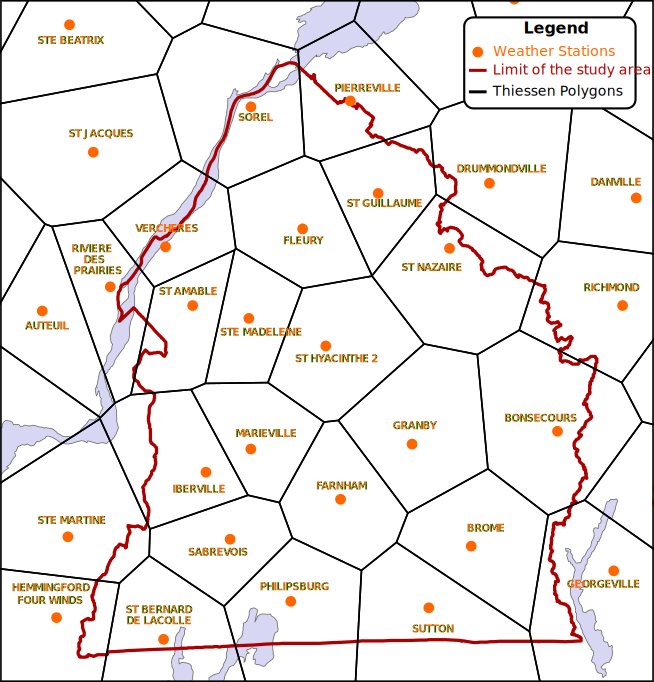
\includegraphics[width=0.45\textwidth]{img/Thiessen_meteo}
    \caption{Spatial distribution of the weather stations in and around the Monteregie Est area, Quebec, Canada.}
    \label{fig:Thiessen_meteo}  
\end{figure}

\begin{figure}[bh!]      
        
    \begin{subfigure}{0.45\textwidth}
        \includegraphics[width=\textwidth]{img/weather_normals_sutton}
        \caption{Sutton Weather Station}
        %\vspace{1em}               
    \end{subfigure} 
    \hspace{0.04\textwidth}   
    \begin{subfigure}{0.45\textwidth}
        \includegraphics[width=\textwidth]{img/weather_normals_nicolet}
        \caption{Nicolet Weather Station}
    \end{subfigure}
    
    \vspace{1cm}   
    
    \begin{subfigure}{0.45\textwidth}
        \includegraphics[width=\textwidth]{img/weather_normals_philipsburg}
        \caption{Philipsburg Weather Station}
        %\vspace{1em}               
    \end{subfigure} 
    \hspace{0.04\textwidth}   
    \begin{subfigure}{0.45\textwidth}
        \includegraphics[width=\textwidth]{img/weather_normals_bonsecours}
        \caption{Bonsecours Weather Station}
    \end{subfigure}
    \caption{Yearly and monthly weather normals for the weather stations with the highest (Sutton) and lowest (Nicolet) annual total precipitation and the warmer (Philipsburg) and colder (Bonsecours) air temperature.}
    \label{fig:weatherNormals}
\end{figure}

\subfile{table_results}

\subsubsection{Air Temperature}

The method gave consistent results for each of the three temperature-related weather variables, for all the 19 weather stations. The RMSE and MAE are both below \SIlist{2.0;1.4}{\celsius} for max ,min, and mean daily air temperature. There is also no bias in the estimations for any of the temperature-based variable with a ME that is, on average for all the stations, less than \SI{0.01}{\celsius} for the max, min, and mean temperature time series. The correlation coefficient between the estimated and measured time series is also above 0.987 for all the weather stations and all the temperature-based variables. The goodness of fit between the estimated and observed values for the max, min, and mean daily temperature are presented for the weather station Granby, located in the center of the study area, in the three graphs of \cref{fig:temp_err}. These graphs are generated automatically at the end of the gap-filling procedure when the cross-validation option is set to \emph{True}.

\begin{figure*}[!bh]
    \begin{subfigure}{0.3\textwidth}
        \includegraphics[width=\textwidth]{img/Max_Temp_(deg_C)}
        \caption{}
        \label{subfig:maxtemp_err} 
    \end{subfigure} 
    \hspace{0.04\textwidth}   
    \begin{subfigure}{0.3\textwidth}
        \includegraphics[width=\textwidth]{img/Min_Temp_(deg_C)}
        \caption{}
        \label{subfig:mintemp_err}                
    \end{subfigure}
    \hspace{0.04\textwidth}
    \begin{subfigure}{0.3\textwidth}
        \includegraphics[width=\textwidth]{img/Mean_Temp_(deg_C)}
        \caption{}
        \label{subfig:meantemp_err}                
    \end{subfigure}
    \caption{Scatter plots comparing the predicted versus the observed daily values for (a) max air temperature, (b) min air temperature, and (c) mean air temperature for the \emph{Granby} weather station.}
    \label{fig:temp_err}
\end{figure*}

\subsubsection{Total Precipitation}

Unlike air temperature, daily precipitation are characterized by high spatial and temporal variability and is thus a weather variable that is more difficult to estimate accurately. Nevertheless, the method gave consistent results for the Monteregie Est region, with a RMSE and MAE that are less than \SIlist{3.4;1.4}{mm} for all the stations. These values are comparable to the results of \cite{xia_forest_1999} and \cite{eischeid_creating_2000} who also used the MLR method to estimate daily precipitation values. The correlation between the estimated and observed daily precipitation is good with values above 0.847 for all the stations. The goodness of fit between the estimated and observed values for the daily total precipitation is presented for the weather station Granby in the graph of \cref{fig:precip_err}

\begin{figure*}[!th]
    \includegraphics[width=0.65\textwidth]{img/Total_Precip_(mm)}
    \caption{Scatter plots comparing the predicted versus the observed daily total precipitation for the \emph{Granby} weather station}
    \label{fig:precip_err}
\end{figure*}

Moreover, from the results of \cref{tab:crossval_restuls}, it can be seen that the differences between the RMSE and MAE are larger for precipitation than for temperature. Moreover, the ME are slightly negatives for 15 of the 19 stations tested. This is due to the fact that regression-based techniques, like the MLR method used in this paper, tend to systematically underestimate heavy precipitation events. This is well demonstrated in \cref{fig:precip_PDF}, where are shown gamma probability density functions that were estimated from the estimated (dashed red line) and observed (solid blue line) daily precipitation time series. The histogram of the distribution of the observed daily precipitation events is also shown on the same figure in light blue. As can be seen, the occurrence of heavy precipitation events is reduced for the estimated time series compared to the measured one. Furthermore, it can also be seen on the graph of \cref{fig:precip_PDF} that the occurrence of zero and light precipitation events is overestimated by the method. This resulted in an overestimation of the number of wet days by \SI{30}{\percent} on average for all the weather stations tested, with a maximal value of \SI{53}{\percent} for the \emph{Vercheres} stations and a minimum value of \SI{13}{\percent} for the \emph{Sutton} station.

The rainfall probability distribution is thus not preserved when using the MLR method. This is a known issue that has been discussed by \cite{simolo_improving_2010}. They also propose a two-step procedure that modifies the MLR method to address both the overestimation of the number of wet days and the underestimation of the heavy precipitation events. Their approach may be incorporated in a future version of the gap-filling algorithm presented in this paper.

\begin{figure}[!th]
    \includegraphics[width=0.65\textwidth]{img/precip_PDF}
    \caption{Gamma probability density functions that were estimated from the estimated (dashed red line) and observed (solid blue line) daily precipitation time series for the \emph{Granby} weather station. The histogram of the distribution of the observed daily precipitation events is also shown in light blue.}
    \label{fig:precip_PDF}
\end{figure}

\end{document}

%The quality of the estimates is strongly affected by seasonality. Stations at higher elevations are difficult to estimate accurately, in large part because of the topographical diversity of the surrounding stations leading to degradation of spatial coherence among stations.

%The tendency for all of the methods to have a negative bias is indicative of the nature of precipitation distributions to be positively skewed (interpolated values will tend to cluster about the median error rather than the mean).

%According to \cite{xia_forest_1999}, the two most important factors in climatology are the inter-correlations in the station network, and the seasonal variations in the relations between the stations.

%An alternative approach would have been to calculate the correlation coefficient with a subset of data from the target series centered around the missing value, as it was done in Simolo et al. (2010) for instance. This approach allows for a better representation of the seasonal variations in the relationships between the stations. The downsides include a more complex algorithm to implement and a reduction of the method robustness and efficiency.